\chapter{Successioni Numeriche}\label{successioni-numeriche}

\defn{Definizione Successione Numerica}{
Si chiama \textbf{successione numerica} una funzione con dominio in $\N$
\[
f: n \in \N \to f(n) \in \R
\]
Si utilizza la seguente notazione: $f(n)=a_{n}\to$ Termine generale della successione.
Una successione si indica o con il suo termine generale $a_{n}$ oppure $\{a_{n}\}_{n\in \N}$.
}

\ex{Esempio 1: $\quad a_{n}=\frac{1}{n}$}
\[
a_{n}=\frac{1}{n} \quad \text{allora} \quad1, \frac{1}{2}, \frac{1}{3}, \frac{1}{4},\dots, \frac{1}{n}
\]

\ex{Esempio 2: $\quad a_{n}=(-1)^n$}
\[
a_{n}=(-1)^n \to -1,1,-1,1,\dots
\]

\ex{Esempio 3: $\quad a_n =n$}
\[
a_n =n \to 1,2,3,\dots
\]

\ex{Esempio 4: $\quad a_{n}=\frac{(-1)^n}{n}$}
\[
a_{n}=\frac{(-1)^n}{n}=-1, \frac{1}{2}, -\frac{1}{3}, \frac{1}{4}, -\frac{1}{5}
\]

\ex{Esempio 5: $\quad a_{n}=-n^2$}
\[
a_{n}=-n^2=-1,-4,-9,-16
\]

\ex{Esempio 6: $\quad a_{n}=\arctan n$}

\ex{Esempio 7: $\quad a_{n}=2^n$}
\[
a_{n}=2^n=1,2,4,8,16,32,64,\dots
\]

\ex{Esempio 8: Formula per il perimetro di un poligono inscritto}
\begin{figure}[H]
    \centering
    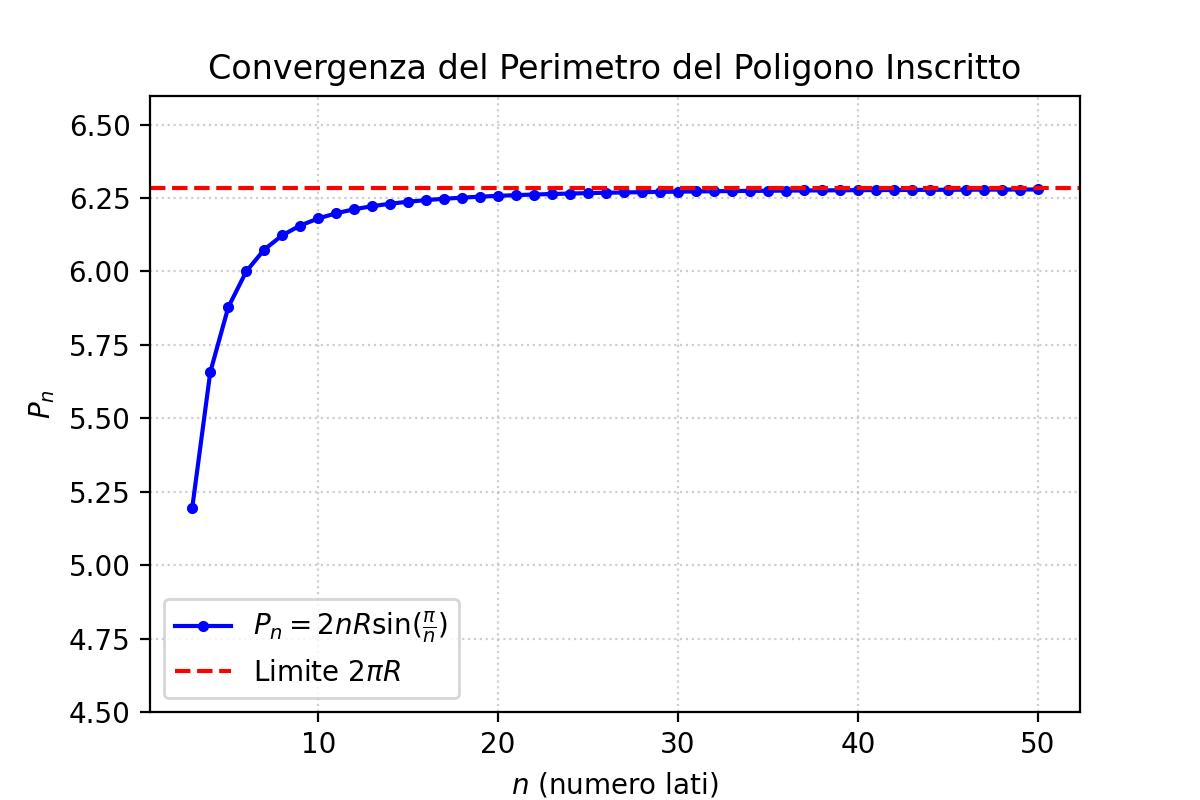
\includegraphics[width=0.6\textwidth]{img/esempio8_succ_numeriche.jpg}
\end{figure}
\[
\begin{aligned}
&P_{n}=n \cdot l\\
&\alpha = \frac{2\pi}{n} \\
&l=2R\sin \frac{\pi}{n} \\
&\boxed{a_{n}=P_{n}=2nR\sin \frac{\pi}{n}} \\
&n\geq3
\end{aligned}
\]

\begin{figure}[H]
    \centering
    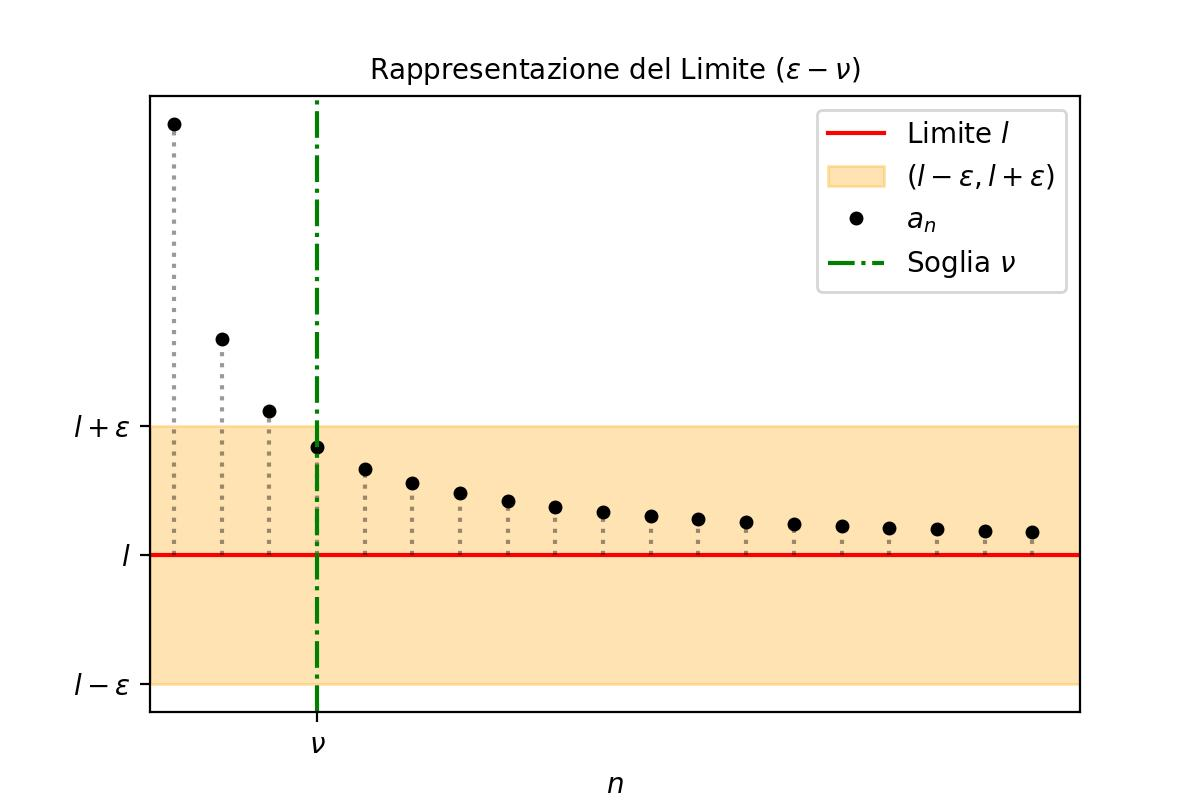
\includegraphics[width=0.8\textwidth]{img/lim_succ_num.jpg}
    \caption{Rappresentazione grafica del limite di una successione.}
\end{figure}

\defn{Definizione Limite di una successione numerica (Convergenza)}{
Assegnata una successione di termine generale $a_{n}$, diremo che $a_{n}$ tende ad $l\in \R$ o che $a_{n}$ converge ad $l\in \R$ se:
\[\forall\epsilon>0\exists \nu>0 :l-\epsilon<a_{n}<l+\epsilon \;\forall n>\nu\]
equivale a dire che:
\[\forall\epsilon>0 \exists \nu>0:|a_{n}-l|<\epsilon \; \forall n > \nu\]
e scriveremo:
\[\boxed{\lim_{ n \to \infty } a_{n}=l}\]
(Posso omettere $+\infty$ nel limite).
\bigskip
(IN PAROLE POVERE):
\begin{itemize}
    \item $\epsilon$ è la larghezza dell'imbuto
    \item $\nu$ è la soglia
    \item $l-\epsilon<a_{n}<l+\epsilon$ è il filtro
\end{itemize}
}

Appunto scollegato:
(a volte con $\nu$)
$x>0,\; x \in \R$
$[x]=$ parte intera (funzione floor())

\section{Limiti di successioni}\label{limiti-di-successioni}

\ex{Esempio 1 — Limite della successione $a_n = \frac{1}{n}$}
\begin{figure}[H]
    \centering
    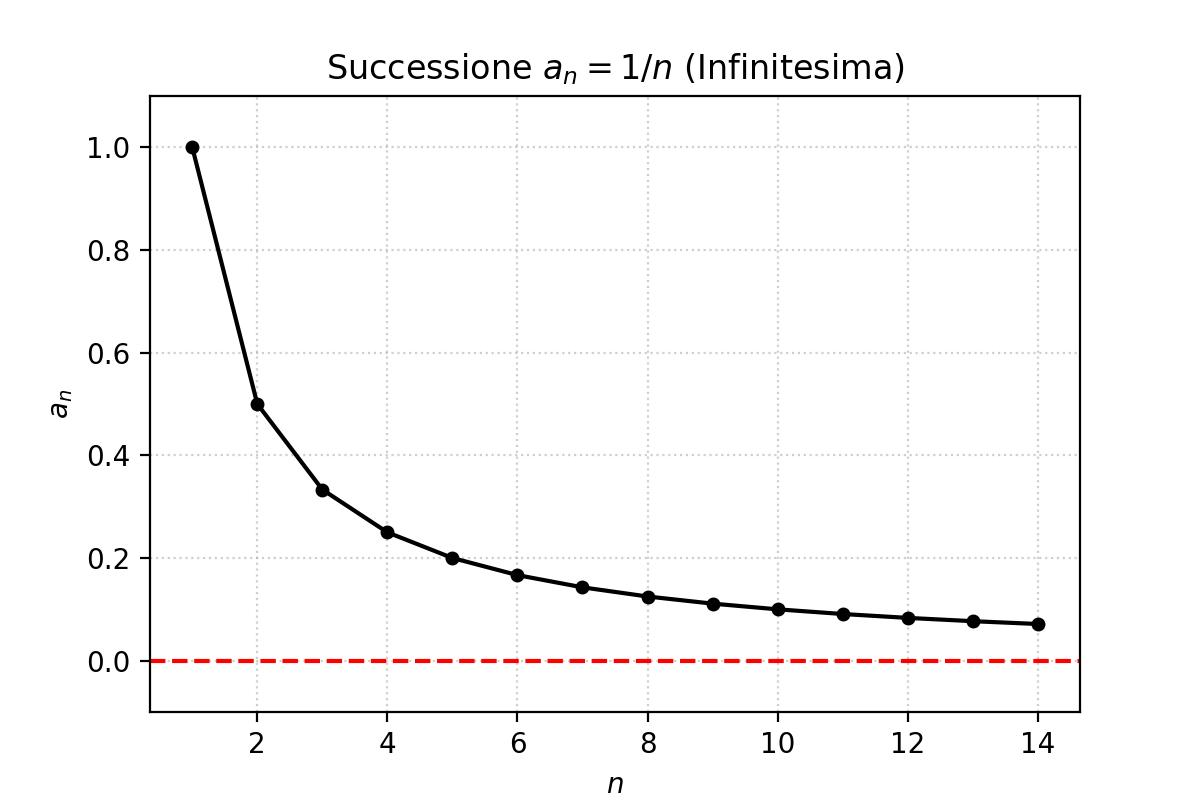
\includegraphics[width=0.8\textwidth]{img/successione_1-su-n.jpg}
    \caption{Successione $a_n = 1/n$.}
\end{figure}

\prop{
\[    
\lim_{n \to \infty} \frac{1}{n} = 0
\]
}

\pf{
Devo dimostrare che:
\[
\forall \, \epsilon > 0 \; \exists \, \nu > 0 \; \text{tale che} \; l - \epsilon < a_n < l + \epsilon \quad \forall n > \nu
\]
Nel nostro caso $l = 0$ e $a_n = \frac{1}{n}$, quindi la condizione diventa:
\[\boxed{-\epsilon < \frac{1}{n} < \epsilon}\]
Poiché $\frac{1}{n} > 0$ per ogni $n$, la disuguaglianza di sinistra è sempre vera. \par
Rimane quindi da imporre:
\[
\frac{1}{n} < \epsilon
\]
da cui segue:
\[
n > \frac{1}{\epsilon}
\]
Poniamo quindi:
\[
\nu = \frac{1}{\epsilon}
\]
Allora, per ogni $n > \nu$, risulta verificata la disuguaglianza \par
\[
-\epsilon < \frac{1}{n} < \epsilon
\]
per ogni $\epsilon > 0$. \par
Quindi:
\[
\boxed{\lim_{n} \frac{1}{n} = 0}
\]
}

\subsection{Successioni Convergenti o Infinitesime}\label{successioni-convergenti-o-infinitesime}

\defn{Definizione}{
Se $a_{n}$ tende ad $l \in \R$ scriviamo anche che: $a_{n}\to l\in \R$
\begin{itemize}
    \item Se $a_{n}\to l\in\R$ diremo che la successione è \textbf{Convergente}.
    \item Se $l=0$ diremo che è \textbf{Infinitesima}.
\end{itemize}
(Non completa tutti i casi):
}

\ex{Esempio 3: $a_n = n$}
\[a_n = n\]
\begin{figure}[H]
    \centering
    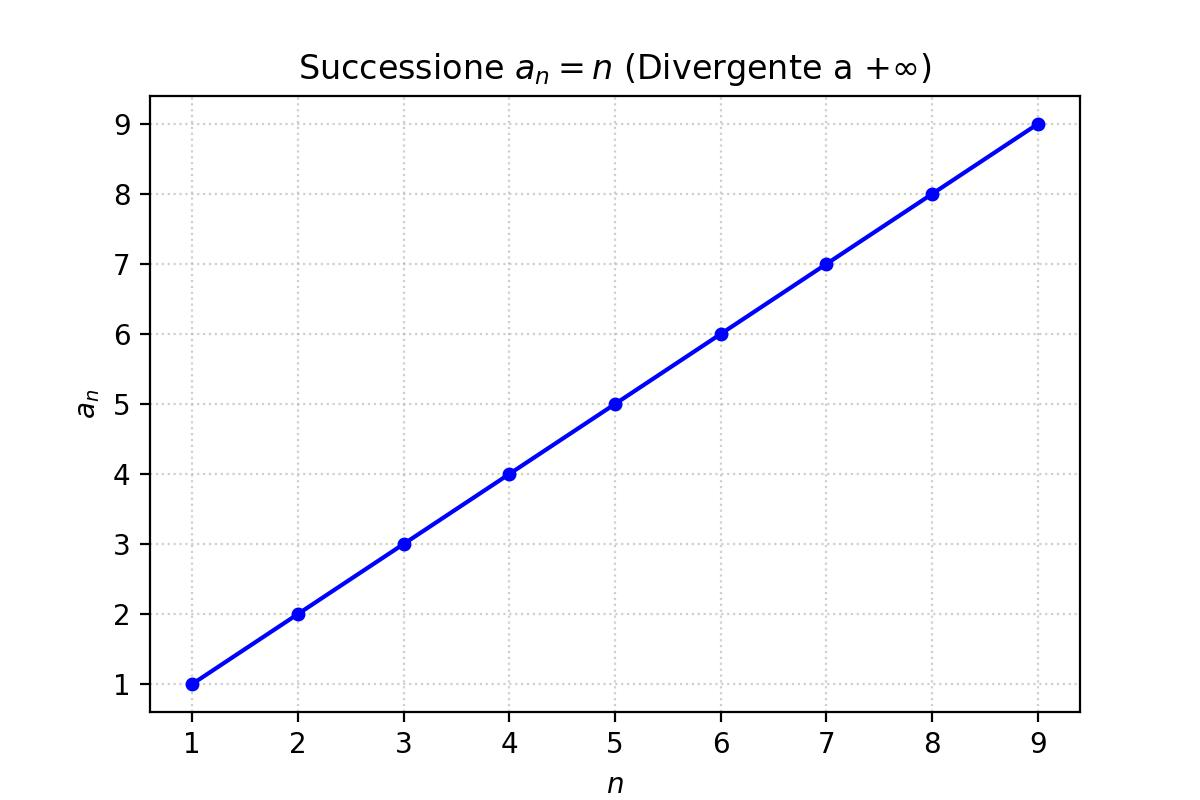
\includegraphics[width=0.6\textwidth]{img/succ_a_n=n.jpg}
    \caption{Successione $a_n=n$.}
\end{figure}

\subsection{Successioni Divergenti}\label{successioni-divergenti}

\defn{Definizione divergenza a $\infty$}{
Assegnata una succesione $a_{n}$ diremo che $a_{n}$ diverge \textbf{POSITIVAMENTE} oppure che diverge o tende a $+\infty$ se:
\[\boxed{\forall M >0 \; \exists \nu >0 : a_{n}>M \quad \forall n>\nu}\]
e scriveremo che:
\[\lim_{ n \to \infty } a_{n}=+\infty \quad\text{ oppure che }\quad a_{n}\to + \infty\]
Diremo che $a_n$ diverge \textbf{NEGATIVAMENTE} oppure che diverge o tende a $-\infty$ se:
\[\boxed{\forall M >0 \; \exists \nu >0 : a_{n}<-M \quad \forall n>\nu}\]
e scriveremo che:
\[\lim_{ n \to \infty } a_{n}=-\infty \quad\text{ oppure che }\quad a_{n}\to - \infty\]
}

\subsection{Successioni regolari o irregolari}\label{successioni-regolari-o-irregolari}

\ex{Esempio 2 - Successione oscillante $a_n = (-1)^n$}
\begin{figure}[H]
    \centering
    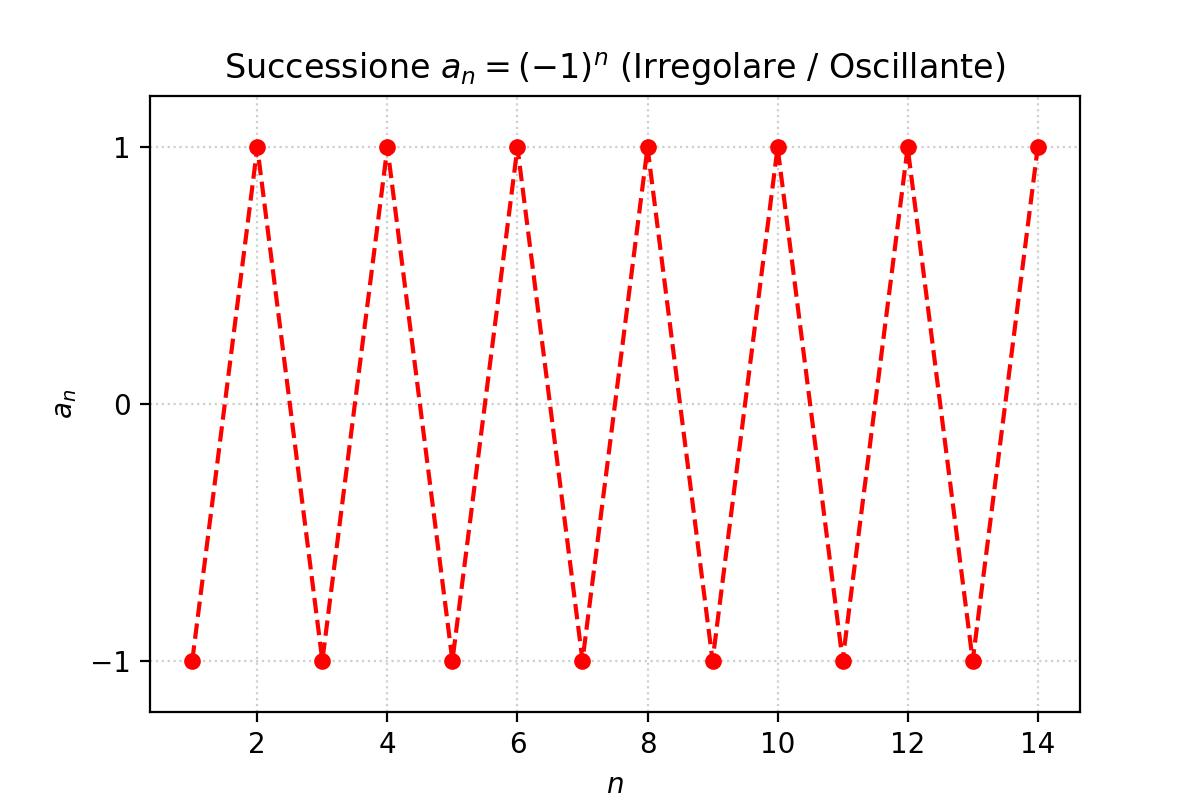
\includegraphics[width=0.6\textwidth]{img/succ_osc_1_-1.jpg}
    \caption{Successione oscillante $a_n = (-1)^n$.}
\end{figure}
Immaginate, per assurdo, che la successione
\[a_n = (-1)^n\]
ammetta un limite.
Allora il limite dovrebbe essere contemporaneamente $1$ (per i termini pari) e $-1$ (per i termini dispari), il che è impossibile.
Quindi:
\begin{itemize}
    \item La successione \textbf{non è convergente}.
    \item Non diverge a $+\infty$ né a $-\infty$.
    \item Questa successione è detta \textbf{irregolare} o \textbf{oscillante}.
\end{itemize}

\defn{Definizione (successione irregolare / oscillante)}{
Sia $a_n$ una successione numerica:
\begin{itemize}
    \item Se $a_n$ \textbf{ammette il limite}, è \textbf{convergente} o \textbf{regolare}.
    \item Se $a_n$ \textbf{non ammette limite} (né finito né infinito), è \textbf{irregolare} o \textbf{oscillante}.
\end{itemize}
}

\section{Definizione di Intorno}

\defn{Definizione Intorno}{
Sia $l \in \R$. Si chiama \textbf{intorno di $l$} qualsiasi intervallo aperto di $\R$ contenente $l$.
\textbf{Esempio:} l'intervallo aperto $]1,\frac{5}{2}[$ è un intorno di $2$.

Un \textbf{intorno di $+\infty$} è, per definizione, una semiretta dx aperta:
\textbf{Esempio:} $]2,+\infty[$.

Analogamente, un \textbf{intorno di $-\infty$} è una semiretta sx aperta:
\textbf{Esempio:} $]-\infty, 2[$.

Gli intorni si possono indicare anche come $I(l)$, $I(+\infty)$, $I(-\infty)$.
}

\prop{
Sia $a_n$ una successione numerica. Allora:
\[
\lim_{n \to \infty} a_n = l \in \overline{\R}
\quad \iff \quad
\forall\, I(l)\; \exists\, \nu \in \N : a_n \in I(l) \quad \forall n > \nu.
\]
}


\pf{Dimostrazione:
La dimostrazione segue direttamente dalla definizione di limite ed è quindi ovvia.
}

\section{Teorema di Unicità del Limite}\label{teorema-unicita-limite}

\defn{Teorema di Unicità del Limite}{
Ogni successione regolare ammette \textbf{UNO e UN SOLO limite}.
}

\pf{Dimostrazione Teorema di Unicità del Limite}{
Si procede per assurdo: \par
Supponiamo che:
\begin{itemize}
    \item $a_n \to l_1 \in \overline{\R}$
    \item $a_n \to l_2 \in \overline{\R}$
\end{itemize}
con $l_1 \neq l_2$.

Essendo $\R$ un campo ordinato, supponiamo senza perdita di generalità che $l_1 < l_2$.
\begin{figure}[H]
    \centering
    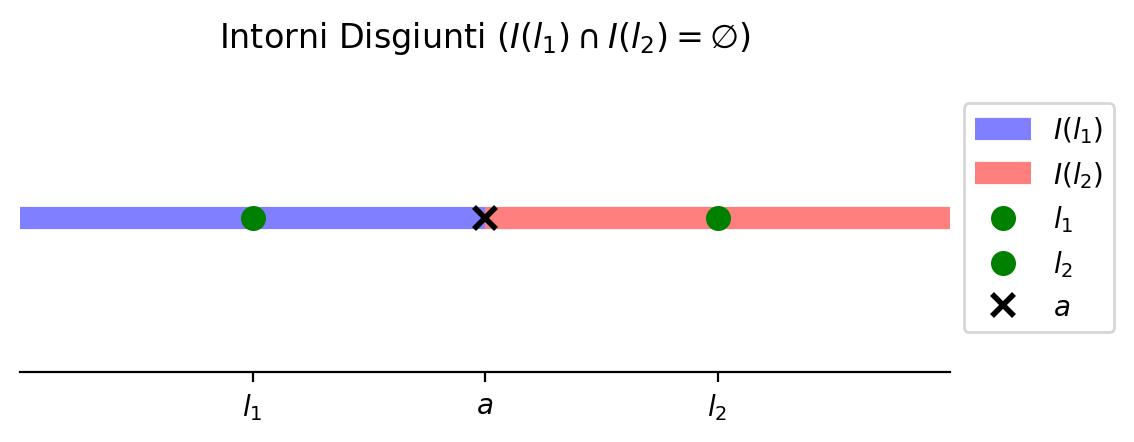
\includegraphics[width=0.8\textwidth]{img/intervalli_unicita_lim.jpg}
    \caption{Intervalli disgiunti per la dimostrazione per assurdo.}
\end{figure}

Poiché $l_1 < l_2$, esiste $a \in \R$ tale che $l_1 < a < l_2$.

Consideriamo gli intorni disgiunti:
\[I(l_1) = ]-\infty, a[, \quad I(l_2) = ]a, +\infty[\]
L'intersezione tra questi due intorni è ovviamente vuota:
\[I(l_1) \cap I(l_2) = \varnothing\]

Per ipotesi, $a_n \to l_1$, allora per questo intorno $I(l_1)$:
\[\exists \, \nu_1 \in \N \; : \; a_n \in I(l_1) \quad \forall n > \nu_1\]
Analogamente, $a_n \to l_2$ allora per questo intorno $I(l_2)$:
\[\exists \, \nu_2 \in \N \; : \; a_n \in I(l_2) \quad \forall n > \nu_2\]

Poniamo:
\[\nu = \max(\nu_1, \nu_2)\]
Allora $\forall n > \nu$, dovremmo avere:
\[a_n \in I(l_1) \cap I(l_2)\]
Ma $I(l_1) \cap I(l_2) = \varnothing$, ASSURDO.
Quindi la nostra ipotesi iniziale era falsa e il limite, se esiste, è \textbf{unico}.
}

\section{Proprietà delle successioni numeriche}

\defn{Definizione Successione Limitata}{
Sia assegnata una successione $a_n$ diremo che è:
\begin{itemize}
    \item \textbf{superiormente limitata} se:
    \[\exists B \in \R : a_n \leq B \quad \forall n \in \N\]
    \item \textbf{inferiormente limitata} se:
    \[\exists A \in \R : A \leq a_n \quad \forall n \in \N\]
    \item \textbf{limitata} se lo è sia inferiormente che superiormente.
\end{itemize}
In quest'ultimo caso:
\[\boxed{A\leq a_n \leq B} \quad \text{oppure} \quad | a_n | \leq M \quad \forall n \in \N\]
}

\rmkb{Osservazione:
Una successione Limitata non per forza converge!!
\ex{Esempio: $(-1)^n$}
$(-1)^n$ è limitata ma oscillante.
}

\prop{
\textbf{Proposizione 1 (Convergenza $\implies$ Limitatezza)} \\
Sia $a_n$ una successione \textbf{convergente}, allora $a_n$ è \textbf{limitata}.
\[
(a_n \text{ convergente } \implies a_n \text{ limitata}) \quad \not\implies \quad
(a_n \text{ limitata } \implies a_n \text{ convergente})
\]
}


\pf{Dimostrazione 1}{
Poichè $a_n \to l \in \R$ per ipotesi, allora $\forall \epsilon > 0 \exists \nu > 0$ tale che:
\[\boxed{l-\epsilon < a_n < l + \epsilon \qquad \forall n > \nu}\]
Sia $\epsilon = 1 \implies \exists \nu > 0:$
\[l-1 < a_n < l +1 \quad \forall n > \nu\]
Ma a noi serve $\forall n \in \N$.
Allora:
\[
E = \{a_1, a_2, a_3, \dots , a_{\lfloor\nu\rfloor}, l-1, l+1 \}
\]
Sia $A = \min E$ e $B = \max E$.
Allora:
\[A \leq a_n \leq B \quad \forall n \in \N\]
}

\prop{
\textbf{Proposizione 2 (Divergenza positiva)} \\
Se $a_n \to +\infty$, allora la successione $a_n$ è \textbf{inferiormente limitata}.
}

\pf{Dimostrazione 2}{
Per hp $a_n \to +\infty$ quindi:
\[\forall M>0 \; \exists \nu > 0 : a_n > M \; \forall n > \nu\]
Considero :
\[
E = \{a_1, a_2, a_3, \dots , a_{\lfloor\nu\rfloor}, M \}
\]
Sia $A = \min E$. Allora per costruzione:
\[a_n \geq A \; \forall n \in \N\]
Ovvero è inferiormente limitata.
}

\prop{
\textbf{Proposizione 3 (Divergenza negativa)} \\
Se $a_n \to -\infty$, allora la successione $a_n$ è \textbf{superiormente limitata}.
\par
La dimostrazione è lasciata come \textbf{esercizio}.
}


\section{Successioni Monotone}

\defn{Definizione — Successioni Monotone}{
Diremo che una successione $a_n$ è:
\begin{itemize}
    \item \textbf{crescente} ($\nearrow$) se $a_n \leq a_{n+1} \quad \forall n \in \N$.
    \item \textbf{strettamente crescente} ($\nearrow_{S}$) se $a_n < a_{n+1} \quad \forall n \in \N$.
    \item \textbf{decrescente} ($\searrow$) se $a_n \geq a_{n+1} \quad \forall n \in \N$.
    \item \textbf{strettamente decrescente} ($\searrow_{S}$) se $a_n > a_{n+1} \quad \forall n \in \N$.
\end{itemize}
}

\ex{Esempi di Monotonia}{
\begin{itemize}
    \item $\frac{1}{n}\;\searrow_{S}$
    \item $n\;\nearrow_{S}$
    \item $\frac{(-1)^n}{n}$ NON è MONOTONA
    \item $2^n \nearrow_{S}$
    \item $a^n \qquad \searrow_{S} \text{ se } 0<a<1 \qquad \nearrow_{S} \text{ se } a>1$
\end{itemize}
}

\prop{
\textbf{Teorema di Regolarità delle Successioni Monotone} \\
Se $a_n$ è una successione \textbf{monotona}, allora $a_n$ è \textbf{regolare} (ammette limite finito o infinito).
}


\defn{Limite di Successioni Monotone}{
Sia $a_n$ una successione monotona. Allora:
\[
\lim_{n \to \infty} a_n =
\begin{cases}
\sup_n a_n & \text{se } a_n \text{ è crescente } (\nearrow) \\
\inf_n a_n & \text{se } a_n \text{ è decrescente } (\searrow)
\end{cases}
\]
}

\ex{Esempi di applicazione}{
\begin{enumerate}
    \item $a_n = \arctan n$ \par
    $a_n \nearrow$, quindi
    \[
    \lim_{n} \arctan n = \sup a_n = \frac{\pi}{2}
    \]
    \item $a_n = \frac{1}{n}$ \par
    $a_n \searrow$, quindi
    \[
    \lim_{n} \frac{1}{n} = \inf a_n = 0
    \]
    \item $a_n = 2^n$ \par
    $a_n \nearrow$, quindi
    \[
    \lim_{n} 2^n = \sup a_n = +\infty
    \]
\end{enumerate}
}

\rmkb{Osservazione sulla Dimostrazione:
La dimostrazione si basa sulle proprietà di sup e inf e sull'assioma di completezza di $\R$.
}

\pf{Dimostrazione Teorema di Regolarità (Caso $a_{n} \nearrow$)}{
Per ipotesi $\boxed{a_{n}\leq a_{n+1}}\;\forall n$ e dobbiamo dimostrare che detto $l=\sup_{n} a_{n}$ allora $\lim_{n \to \infty} a_{n}=l$.
\par
DUE CASI:
\begin{enumerate}
    \item \textbf{Caso 1 ($l<+\infty$):}
    Dobbiamo dimostrare che:
    \[
    \boxed{\forall \epsilon >0 \exists \nu : l-\epsilon < a_{n} <l+\epsilon \quad \forall n > \nu }
    \]
    Sia $\epsilon$ fissato. Per la proprietà dell'estremo superiore, si ha che $\exists \nu \in \N$ tale che $l-\epsilon < a_{\nu}$.
    Poiché $a_n$ è crescente, per ogni $n > \nu$ si ha $a_n \geq a_\nu$. Inoltre, $l$ è l'estremo superiore, quindi $a_n \leq l$.
    Quindi, per $\forall n > \nu$:
    \[
    l-\epsilon < a_{\nu} \leq a_{n} \leq l < l+\epsilon \quad (\text{tesi})
    \]

    \item \textbf{Caso 2 ($l=+\infty$):}
    Dobbiamo dimostrare che:
    \[
    \boxed{\forall M > 0 \exists \nu > 0 : a_{n} > M \quad \forall n > \nu}
    \]
    Usiamo la proprietà del $\sup a_{n} = +\infty$: $\forall M > 0 \exists \nu \in \N$ tale che $a_{\nu} > M$.
    Poiché $a_n$ è crescente, $\forall n > \nu$ si ha $a_{n} \geq a_{\nu} > M$, da cui la tesi.
\end{enumerate}
La dimostrazione per $a_{n} \searrow$ è analoga.
}

\rmkb{Osservazione sulla Convergenza:
$a_{n}$ è monotona + limitata $\implies a_{n}$ convergente
}

\subsection{Proprietà definitivamente vera}

\defn{Definizione Proprietà Definitivamente Vera}{
Una proprietà che dipende da $n \in \N$ si dice \textbf{DEFINITIVAMENTE} vera se vale da un certo indice $n$ in poi.
}

\rmkb{Osservazione sulla Regolarità:
Nel Teorema di Regolarità, posso scrivere: "Se $a_n$ è una successione definitivamente \textbf{monotona}, allora $a_n$ è \textbf{regolare}."
}

\prop{
\textbf{Proposizione (Valore Assoluto)} \\
Se $a_n$ è una successione \textbf{convergente} e $a_n \to l$, allora vale:
\[
|a_n| \to |l|.
\]
}


\pf{Dimostrazione Valore Assoluto}{
Si usa la disuguaglianza triangolare inversa: $|a-b|\geq ||a|-|b||$.
\[||a_{n}|-|l||< |a_{n} -l |<\epsilon \quad \forall n > \nu\]
}

\prop{
\textbf{Proposizione (Infinitesima)} \\
Si ha che:
\[
a_n \to 0 \quad \iff \quad |a_n| \to 0.
\]
}


% DA TERMINARE (? sul quaderno)